
% VYSOKOŠKOLSKÁ KVALIFIKAČNÍ PRÁCE
% autor: Michal Struna
% název: Umělá inteligence pro detekci exoplanet

\documentclass[a4paper,12pt]{article}

\usepackage{utils}
\usepackage{titletoc}
\usepackage{amssymb}  % TODO: Odebrat
\usepackage{amsmath}

\def\code#1{\texttt{#1}}


\expandafter\def\expandafter\UrlBreaks\expandafter{\UrlBreaks%  save the current one
  \do\-}


% ÚDAJE O PRÁCI
\def\jmenoFakulty{Fakulta elektrotechniky a informatiky}
\def\jmenoAutora{Michal Struna}
%\def\nazevPrace{Umělá inteligence pro detekci exoplanet}
%\def\nazevPrace{Distribuované výpočty a umělá inteligence\\ pro detekci a analýzu exoplanet}
\def\nazevPrace{Detekce a~analýza exoplanet s~využitím\\distribuovaných výpočtů a~umělé inteligence}
\def\typPrace{Diplomová práce}
\def\rok{2021}
\def\prefixZadani{img/zadani}	% cesta a začátek jména, bude doplněno číslo strany
\def\suffixZadani{.jpg}		% doplní se ke každému jménu souboru zadání
\def\datumOdevzdaniPrace{9.\,5.\,2021}

\long\def\textPodekovani{...}


\long\def\anotace{
...
}
\def\klicovaSlova{exoplanety, extrasolární planety, kepler, umělá inteligence, python}
\def\title{Artificial intelligence for exoplanet detection from transit data}
\long\def\annotation{
...
}
\def\keywords{exoplanet, extrasolar planets, kepler, artificial intelligence, python}

%%%%%%%%%%%%%%%%%%%%%%%%%%%%%%%%%%%%%%%%%%%%%%%%%%%%%%%%%%%%
% ZAČÁTEK DOKUMENTU
%%%%%%%%%%%%%%%%%%%%%%%%%%%%%%%%%%%%%%%%%%%%%%%%%%%%%%%%%%%%

\begin{document}

\deskpage
\mainpage
\assignment
\statement
\acknowledgment
\annotationcs	
\annotationen
\content
\imglist
\tablelist
\codelist
\formulalist
\shortlist

\begin{description}[font=\mdseries,leftmargin=6em,labelwidth=!,]
\item[CNN]      Convolutional neural network
\item[csv]      Comma-separated values
\item[FC]       Fully-connected layer
\item[FFNN]     Feed-forward neural network
\item[fits]     Flexible image transport system
\item[ly]		Light year
\item[au]		Astronomical unit
\end{description}

\clearpage\pagestyle{plain}\phantomsection\addcontentsline{toc}{section}{Úvod}
\section*{Úvod}
\label{uvod}

V naší sluneční soustavě se nachází celkem 8 dosud objevených planet včetně Země. Mimo ni ale v~pozorovatelném vesmíru existují odhadem stovky miliard galaxií a~v~každé z~nich v~průměru stovky miliard hvězd. Z toho, co o~vzniku a~fungování hvězdných soustav víme je pravděpodobné, že většinu těchto hvězd bude obíhat jedna nebo více planet, tzv. extrasolárních planet nebo také exoplanet.~\cite{exoplanets}

První potvrzená exoplaneta byla objevena již roku 1992, ale výzkum exoplanet se dostal do oblasti širokého zájmu až během posledního desetiletí. Stalo se tak především kvůli vesmírnému teleskopu Kepler, který má na svém kontě od roku 2009 přes 2~500 objevených exoplanet. [TODO]

K~dnešnímu dni je známo více jak 4 000 potvrzených exoplanet. Toto číslo se s~nejvyšší pravděpodobností bude rychle zvyšovat, protože roku 2018 byl vypuštěn nástupce Kepleru -- satelit TESS -- od něhož je očekáván objev 20~000 exoplanet.~\cite{tess}

Planety u~jiných hvězd většinou nelze pozorovat přímo. Proto je nepřímými metodami zkoumáno jejich působení na své mateřské hvězdy, které už pozorovat lze. Výstupem z~takovýchto pozorování jsou často stovky GiB fyzikálních a~statistických dat, jež je následně nutno zpracovat.~\cite{exoplanets}

Cílem této diplomové práce je vytvořit aplikaci umožňující uživatelům poskytovat výpočetní výkon svých počítačů pro analýzu právě těchto dat. Projekt sestává z~klientského programu, webové aplikace a~serveru. Klientský program provádí potřebné distribuovatelné výpočty na počítači uživatele. Tento program je možné ovládat z~rozhraní webové aplikace, jež zároveň poskytuje přehled o~všech aktivitách, uživatelích a datech. Rozdělování výpočetních úloh mezi klienty a~ukládání dat do databáze pak řeší server.

Díky distribuovaným výpočtům se do výzkumu exoplanet bude moci bez vysokého úsilí, znalosti či technického vybavení zapojit i široká veřejnost. To může urychlit vývoj a zároveň zvýšit povědomí o~této vědní disciplíně.

V~projektu jsou využity některé techniky spadající pod umělou inteligenci, v~důsledku čehož je zpracovávání dat zcela automatizované. Platí však, že umělá inteligence je v~současnosti stále intenzivně se rozvíjející oblastí, a~proto výsledky nemusí být natolik vypovídající ve srovnání s~tím, kdy by výzkum prováděli lidé manuálně, byť by to trvalo nesrovnatelně déle.

\section{Exoplanety}

\subsection{Důvody hledání}

TODO

\subsection{Typy exoplanet}

TODO

\subsection{Objevené exoplanety}

TODO

\section{Metody hledání exoplanet}

Exoplanety není téměř vůbec možné pozorovat přímo vizuálně, protože neemitují žádné světlo a~nachází se ve velkých vzdálenostech od Země. Lze ovšem pozorovat jejich působení na blízké hvězdy nebo jiné viditelné útvary. K~tomuto účelu se používá několik metod popsaných v této kapitole.

Zdaleka nejvýznamnější je tranzitní metoda, kterou byla objevena většina exoplanet. Velké množství planet bylo objeveno taktéž metodou radiálních vzdáleností. Pomocí ní byly objevovány planety především blízko Země.~\cite{nasadata}

\img[1]{Počty objevených exoplanet jednotlivými metodami}{stats/count_by_method.png}

\data{1}{nasadata}

Málo hmotné planety byly objevovány častěji tranzitní metodou, zatímco hmotnější planety spíše metodou radiálních rychlostí. Pro planety vzdálené od své mateřské hvězdy se nejlépe osvědčila metoda přímého zobrazení.~\cite{nasadata}

\img[1]{Závislost hmotnosti, periody oběhu a metody objevení planety}{stats/period_by_mass_by_method.pdf}

\data{1}{nasadata}

\clearpage
\subsection{Tranzitní metoda}

Někdy se planeta při obíhání dostane mezi svou hvězdu a~Zemi. Tento jev se pro pozorovatele na Zemi projeví jako mírný pokles jasu hvězdy (obvykle ve zlomku procenta). Pokud je hvězda teleskopem sledována dlouhodobě, je možné v~těchto změnách jasu hvězdy odhalit opakující se složku. To by mohlo indikovat přítomnost planety v~blízkosti této hvězdy.~\cite{exoplanets,transit}

\img[1]{Přechod planety přes kotouč hvězdy}{img/transit.png}
\drawgimp

Tyto změny však nemusí být na první pohled viditelné, protože v~soustavě může být více planet, které svou hvězdu zastiňují různou měrou a~obíhají kolem ní s~různou periodou. Navíc i v situaci, kdy je ve změnách jasu hvězdy objevena periodická složka nemusí jít vždy o~obíhající planetu. Hvězda může být např. sama o~sobě proměnlivá nebo se může jednat o~dvojhvězdu, jejíž složky se vzájmně zastiňují.~\cite{kepler80}

Tranzitní metoda vzbuzuje velký zájem především kvůli možnosti objevovat i~malé planety podobné Zemi~--~takové planety by mohly spíše splňovat podmínky pro život. Nevýhodou je, že většina exoplanet obíhá svou hvězdu v~takové rovině, v jaké pozorovatel na Zemi nemůže transit spatřit. Odhadem 99 \% všech potenciálních exoplanet podobných Zemi nemůže být tranzitní metodou nikdy zachyceno.~\cite{methods,transit}

\formula{Pravděpodobnost zpozorování tranzitu planety přes hvězdu} {P = \frac{d_s}{a}}{
\begin{tabular}{llll}
	$d_s$ = průměr hvězdy & a = vzdálěnost exoplanety od hvězdy \
\end{tabular}
}

%\img[1]{xxx}{http://hvezdy.astro.cz/obr/hvezdy/exoplanety/geometrie.jpg}

\subsubsection{Target pixel file}

Prvním krokem v~analýze hvězdy tranzitní metodou je její fyzické pozorování. Teleskop obvykle pozoruje část oblohy po dobu několika měsíců, přičemž každých několik desítek minut vytvoří snímek dané části oblohy. Z~výsledných fotografií se následně vyextrahují jednotlivé hvězdy, čímž vzniknou tzv. target pixel files.

TPF obsahuje část oblohy o velikosti několika pixelů, na které se v původní fotografii nacházela zkoumaná hvězda a~její okolí. Barva pixelů je určena jasem.

\img[1]{Target pixel file hvězdy Kepler-10}{img/tpf.png}
\data{1}{nasadata}

\subsubsection{Světelná křivka hvězdy}

Po složení všech TPF do časové řady a~vypočítání jejich jasu dostaneme světelnou křivku. Na obrázku~5 je světelná křivka hvězdy Kepler-13 očištěná od dlouhodobého trendu, šumu a~extrémních hodnot. Křivka vykazuje velice výraznou periodickou složku s~periodou 1,763~dne. Ve většině případů ale vliv planety není takto výrazný a~detekovat planetu je obtížnější.

\img[1]{Světelná křivka soustavy Kepler-13}{img/light_curve.png}
\data{1}{nasadata}

Každý tranzit má charakteristické fáze, které pomohou odlišit působení exoplanety od ostatních možných příčin, jako je např. proměnlivost hvězdy, dvojhvězda nebo pulzar.


\img[1]{Detail světelné křivky soustavy Kepler-13}{img/light_curve_detail.png}

\begin{enumerate}
\item Planeta je schovaná za hvězdou, hvězda je vidět se svým základním jasem.
\item Planeta je vedle hvězdy, jas hvězdy je posilněn o~světlo odražené od planety.
\item Planeta je vedle hvězdy, ale její viditelná část není osvětlena. Hvězda je vidět se svým základním jasem.
\item Planeta je před hvězdou, jas hvězdy je snížen v~důsledku zakrytí části kotouče.
\end{enumerate}

Tyto fáze společně s~důležitými parametry tranzitu potřebnými pro další výpočty jsou vyznačeny na obrázku~6:

\begin{enumerate}[label=\Alph*.]
\item Perioda -- čím větší perioda, tím delší planetární rok a větší velká poloosa dráhy,
\item Hloubka -- čím větší hloubka, tím je planeta vůči hvězdě větší,
\item Trvání -- čím je trvání kratší, tím menší trajektorii přes hvězdu planeta má,
\item Délka nástupu -- čím prudší a~kratší je nástup, tím menší je úhel mezi rovinou orbity exoplanety a~přímkou od hvězdy k~pozorovateli,
\item Délka minima -- čím větší délka minima v~porovnání s~délkou transitu, tím je úhel mezi rovinou orbity exoplanety a~přímkou od hvězdy k~pozorovateli menší.
\end{enumerate}

\subsubsection{Vyřazení false positives}

Většina periodických složek ve světelných křivkách hvězd jsou \emph{false positive}~--~patří jiným jevům, než je obíhající planeta. Tyto případy je třeba odfiltrovat, což byla až donedávna především manuální práce lidí -- vědců či dobrovolníků. Protože ale tranzit planety vykazuje specifický průběh popsaný v předchozí kapitole, je možné ho s~určitou úspěšností rozpoznat pomocí naučené umělé neuronové sítě automaticky.~\cite{kepler80}

\begin{multicols}{2}
\img[1]{Dvojhvězda KIC~8262223}{img/eclipsing_binary.png}
\img[1]{Cefeida KIC 3733346}{img/cepheid.png}
\end{multicols}

\begin{multicols}{2}
\img[1]{Proměnná hvězda KIC~9832227}{img/variable_star.png}
\img[1]{Kataklizmická proměnná hvězda KIC 9406652}{img/cataclysmic.png}
\end{multicols}

\data{1}{nasadata}

Je třeba aby vstupní data do neuronové sítě měla stejné rozměry i~formát. Vzhledem k~různorodosti světelných křivek je nutno provést několik kroků, abychom dosáhli standardizovaného formátu. Prvním krokem je složení časové řady do jedné periody, čímž dojde k~posílení viditelnosti transitu (pokud zde nějaký je), nebo naopak k~jeho vyrušení (pokud zde žádný není).~\cite{kepler80}

\begin{multicols}{2}
\img[1]{Světelná křivka Kepler-10}{img/full_light_curve.png}
\img[1]{Složená světelná křivka}{img/folded.png}
\end{multicols}

Na obrázku 12 je uprostřed slabě patrný transit. Má malou šířku, protože trvá pouze 0,25 dne, zatímco celá perioda je dlouhá 45,3 dne. Z~této složené časové řady se vytvoří dva pohledy, které budou vstupem do neuronové sítě:

\begin{itemize}
\item \textbf{Globální pohled} \emph{(obr. 13)} -- Šířka periody a~počet bodů v~časové řadě jsou fixní. Nevýhodou je, že u planet s~dlouhou periodou bude tranzit velice nepatrný, proto pouze globální pohled nestačí.~\cite{kepler80}
\item \textbf{Lokální pohled} \emph{(obr. 14)} -- Šířka tranzitu a počet bodů v časové řadě jsou fixní. Nevýhodou je, že není viditelný celý průběh světelné křivky. Naproti tomu je ale zřetelný tranzit.~\cite{kepler80}
\end{itemize}

\begin{multicols}{2}
\img[1]{Globální pohled na tranzit Kepler-10~c}{img/global_view.png}
\img[1]{Lokální pohled na tranzit Kepler-10~c}{img/local_view.png}
\nasa
\end{multicols}

Fixní počet bodů lze zajistit nahrazením každých $\frac{\alpha}{\beta}$ sousedních bodů ($\alpha$ -- současný počet bodů, $\beta$ -- požadovaný počet bodů) jediným, který bude reprezentovat jejich medián. Pro potřeby neuronové sítě je nutno oba pohledy taktéž normalizovat tak, aby platilo $H~=~\left<1; -1\right>$. U~případů, které neuronová síť vyhodnotí jako planety, je možné pokračovat výpočtem dalších informací o~planetě.~\cite{kepler80}

\subsubsection{Výpočet vlastností planety}

Velkou poloosu dráhy planety lze vypočítat, pokud známe hmotnost hvězdy a periodu oběhu z~třetího Keplerova zákona.~\cite{transitprops}

\formula{Výpočet velké poloosy dráhy planety}{a = \sqrt[3]{\frac{GMP^2}{4\pi^2}}}{
\begin{tabular}{llll}a = velká poloosa & G = gravitační konstanta & M = hmotnost hvězdy & P = perioda oběhu planety\end{tabular}
}

Ze světelné křivky a~poloměru hvězdy lze vypočítat poloměr tranzitující planety po vyjádření z~následující rovnice~\cite{transit,transitprops}:

\formula{Výpočet poloměru planety} {\frac{r^2}{R^2} = \frac{\Delta F}{F}}{
\begin{tabular}{llll}
	r = poloměr planety & R = poloměr hvězdy & F = jas hvězdy & $\Delta F$ = změna jasu \
\end{tabular}
}

Dále je možno odhadnout i~průměrnou rychlost pohybu planety po oběžné dráze. Skutečná průměrná rychlost však může být jiná, protože se nepočítá s excentricitou dráhy~\cite{transitprops}:

\formula{Odhad průměrné rychlosti oběhu planety}{v \approx \frac{2\pi a}{T}}{
\begin{tabular}{lll}
    v = rychlost oběhu planety & a = velká poloosa dráhy planety & T = perioda oběhu planety
\end{tabular}
}

Další z~důležitých charakteristik orbity je inklinace (sklon), která nám řekne, jaký úhel svírají roviny pozorovatele a~oběhu exoplanety. Bohužel lze zjistit minimální úhel sklonu dráhy a~nikoliv jeho přesnou hodnotu. Inkinace se bude zpravidla blížit 90$^{\circ}$.~\cite{transitprops}

\formula{Výpočet inklinace dráhy}{\cos{i} \leq \frac{R + r}{a}}{
\begin{tabular}{llll}
    i = inklinace & R = poloměr hvězdy & r = poloměr planety & a = velká poloosa dráhy planety
\end{tabular}
}

\subsubsection{Výpočet hmotnosti planety}

Hmotnost planety z~tranzitní metody nelze vypočítat. Avšak z~empirických dat je možné ji odhadnout na základě kombinace jiných veličin pomocí umělé neuronové sítě. TODO.~\cite{nnmass}

\clearpage
\subsection{Metoda radiálních rychlostí}

Stejně jako hvězda ovlivňuje obíhající planetu, tak i~planeta gravitačně ovlivňuje svou hvězdu a~obě tělesa obíhají kolem společného těžiště. Tento pohyb se může projevit jako opakované přibližování a~vzdálování hvězdy vůči pozorovateli na Zemi. Právě pojem radiální rychlost označuje rychlost pohybu ve směru přímky k~pozorovateli.~\cite{methods}

Pokud se zdroj elektromagnetického záření (hvězda) přibližuje vůči pozorovateli, záření má menší vlnovou délku a~jeví se více do modra, protože právě modrá (a~fialová) barva má z~viditelného spektra nejmenší vlnovou délku. Obdobná situace nastává při vzdálování se zdroje vlnění od pozorovatele. Vlnová délka se zvětšuje a~barva jde do červena. Tomuto efektu se říká červený (resp. modrý) posuv.~\cite{methods}

\img[1]{Metoda radiálních vzdáleností}{img/radial_velocity.png}
\drawgimp

Příčinou červeného/modrého posuvu je v~tomto případě Dopplerův jev, který lze uplatnit i pro jiné druhy vlnění, než to elektromagnetické~--~zvuk. Pokud se k~nám zdroj zvuku přibližuje (např. siréna na jedoucím autě), zvuk zpravidla vnímáme vyšším tónem, protože má menší vlnovou délku (vyšší frekvenci). Při vzdalování zdroje má zvuk větší vlnovou délku a je vnímán hlubším tónem.~\cite{radialvelocity}

Periodicky se opakující změny ve vlnové délce záření hvězdy tak mohou být důsledkem existence tělesa v této soustavě.~\cite{methods}

\subsubsection{Měření vlnové délky záření hvězdy}

Hvězdy nevyzařují světlo pouze jedné jediné vlnové délky, nýbrž celé spektrum. Tento efekt lze vidět  u~duhy v~zemské atmosféře, kdy jsou jednotlivé složky slunečního světla odděleny. Záření z~hvězd se dokonce neomezuje pouze na viditelné světlo, ale pokrývá značnou část celého elektromagnetického spektra. Jak velká část záření přísluší jednotlivým vlnovým délkám lze měřit pomocí spektrometru.~\cite{radialvelocity, sunlight}

\img[1]{Spektrum slunečního záření}{stats/sunlight_spectrum.png}
\data{1}{sunlight}

Změna vlnové délky záření se projevuje jako horizontální posun barevného spektra hvězdy. Nutno podotknout, že zemská atmosféra některé vlnové délky pohlcuje. Proto i~přesto, že Slunce má barvu spíše do zelena vidíme tuto hvězdu ze Země žlutě. [TODO]

\subsubsection{Výpočet radiální rychlosti hvězdy}

Poté, co teleskop sesbírá dostatečně velkou časovou řadu vlnových délek záření hvězdy může dojít k~vypočítání změn radiální rychlosti v~čase. Lze tak učinit dle vzorce~3. Platí, že radiální rychlost je kladná, pokud se zdroj od pozorovatele vzdaluje a~záporná pokud se přibližuje.~\cite{methods}

\formula{Radiální rychlost na základě změny vlnové délky} {v = c * \frac{\Delta\lambda}{\lambda_0}}{
\begin{tabular}{lll}
	$\Delta\lambda$ = změna vlnové délky & $\lambda_0$ = klidová vlnová délka & v = radiální rychlost \
\end{tabular}
}

Graf znázorňující radiální rychlost hvězdy 51~Pegasi může vypadat takto:

\img[1]{Radiální rychlost hvězdy 51 Pegasi}{stats/51_pegasi_radial_velocity.pdf}
\data{1}{51pegasi}

Na první pohled je patrná jedna periodická složka s periodou 4,23 dne a~amplitudou 56,04 $\frac{m}{s}$, která značí, že kolem této hvězdy obíhá jedna planeta. Pokud zde jsou přítomna i~jiná tělesa, důvodů, proč je metoda radiálních rychlostí neodhalila může být několik:

\items{
\item Hmotnost tělesa je vůči hmotnosti hvězdy zanedbatelná,

\item Perioda oběhu tělesa je příliš velká (desítky let a~více), a~proto se ji nepodařilo zachytit na tak krátkém časovém úseku,

\item Těleso obíhá po dráze, jejíž rovina je kolmá k~přímce směrem~k pozorovateli (k Zemi). To vede k~tomu, že je hvězda vychylována takovým směrem, který nemá vliv na radiální rychlost hvězdy vůči Zemi.
}

\subsubsection{Výpočet hmotnosti planety}

Hlavní výhodou metody radiálních rychlostí oproti tranzitní metodě je možnost spočítat hmotnost exoplanety. Její přesnou hodnodu však lze odvodit pouze se znalostí sklony dráhy exoplanety vůči pozorovateli. V~opačném případě lze vypočítat pouze dolní mez hmotnosti planety, a~to zejména kvůli $M_p * sin(i)$ ve vzorci 5.~\cite{methods}

\formula{Radiální rychlost}{\Delta v_{max} = \sqrt[3]{\frac{2\pi G}{T}} * \frac{M_p * sin(i)}{\sqrt[3]{(M_p + M_s)^2}} * \frac{1}{\sqrt{1 - e^2}}}{
\begin{tabular}{lll}
	$\Delta v_{max}$ = amplituda změny rychlosti & $M_s$ = hmotnost hvězdy & $M_p$ = hmotnost planety \\
	sin(i) = sklon dráhy vůči pozorovateli & e = excentricita dráhy & T = oběžná doba \\
\end{tabular}
}

V tabulce 2 jsou uvedeny příklady výpočtu hmotnosti některých planet.

{ % TODO
\catcode`\-=12
\tab[1]{Příklady výpočtu hmotnosti planet}{
	\begin{tabular}{|l|l|l|l|l|l|l|l|}
		\hline	
		\rowcolor{lightgray}
		Těleso & Hvězda & $\Delta v_{max}$ [$\frac{m}{s}$] & $M_p$ [kg] & sin(i) & e & T [r] & \textbf{$M_s$ [kg]} \\
			
		\hline	
		Země & \multirow{3}{*}{Slunce} & 0,089 & \multirow{3}{*}{$2 * 10^{30}$} & \multirow{5}{*}{1} & 0,017 & 1 & \textbf{$5,97 * 10^{24}$} \\
		
		\cline{1-1}\cline{3-3}\cline{6-8}
		Jupiter & & 12,4 & & & 0,048 & 11,86 & \textbf{$1,9 * 10^{27}$} \\
		
		\cline{1-1}\cline{3-3}\cline{6-8}
		\cline{1-1}\cline{3-3}\cline{6-8}
		Pluto & & 0,00003 & & & 0,247 & 247,41 & \textbf{$1,3 * 10^{22}$} \\
		
		\cline{1-1}\cline{3-3}\cline{6-8}
		\cline{1-4}\cline{6-8}


		$\alpha$ Cen Bb & $\alpha$ Cen B & 0,51 & $1,8 * 10^{30}$ & & 0 & 0,0089 & \textbf{$6,75 * 10^{24}$} \\	
		\cline{1-4}\cline{6-8}
		51 Pegasi b & 51 Pegasi & 55,9 & $2,22 * 10^{30}$ & & 0,013 & 0,0116 & \textbf{$0,88 * 10^{27}$}  \\		
		\hline
	\end{tabular}
}

\data{1}{radialvelocity, 51pegasi, methods, nasadata}

\clearpage
\subsection{Astrometrická metoda}

Astrometrická metoda využívá stejné vlastnosti vzájemného působení těles jako metoda radiálních rychlostí. Namísto zkoumání vlnové délky záření se však zaměřuje na polohu hvězdy. Hvězda, kolem níž obíhá dostatečně hmotné těleso, se bude v~důsledku působení tělesa nepatrně vychylovat ze své pozice~--~bude obíhat kolem těžiště soustavy.~\cite{methods}

\img[1]{Astrometrická metoda}{img/astrometry.png}

Pohyb hvězdy tak není přímočarý, ale vlnitý. Kolísání hvězdy je však pro pozorovatele na Zemi často pouze v~řádu stovek úhlových mikrovteřin až jednotek milivteřin.~\cite{methods} Z~tohoto důvodu byla astrometrickou metodou dosud objevena pouze jediná exoplaneta.~\cite{nasadata}

\img[1]{Kolísání hvězdy Gliese~876~s~planetou}{img/astrometry_trajectory.png}
\drawgimp

Dá se však očekávat, že se zlepšující se technikou bude tato metoda úspěšnější.

\subsection{Gravitační mikročočky}
\subsection{Přímé zobrazení}
\subsection{Transit timing}
\subsection{Pulsar timing}

\section{Umělá inteligence}

\subsection{Umělé neuronové sítě}

\subsection{Evoluční algoritmy}

\subsubsection{Genetický algoritmus}

\subsubsection{Algoritmus diferenciální evoluce}

\subsection{Fuzzy systémy}

\subsection{Expertní systémy}

\section{Umělé neuronové sítě}

Jednou z~oblastí patřících do oboru umělé inteligence jsou umělé neuronové sítě, jež se inspirovaly biologickými neuronovými sítěmi. Jejich použití je vhodné na problémy, u~kterých neexistuje přesný matematický popis řešení nebo sice existuje, ale jeho realizace by byla příliš složitá. Hlavními oblastmi, kde se neuronové sítě využívají, jsou např.:

\begin{itemize}
\item \textbf{Predikce} (předpověď počasí,  vývoj cen akcií na burze, ...),

\item \textbf{Rozpoznávání vzorů} (rozpoznávání ručně psaného textu, detekce tranzitu planety ve světelné křivce hvězdy, ...),

\item \textbf{Analýza nebo transformace signálů} (odstranění šumu ze signálu, komprese, převod psaného textu na mluvený signál, ...),

\item \textbf{Řízení v~dynamicky se měnících podmínkách} (autopilot, ...).~\cite{nn}

\end{itemize}

\subsection{Neuron}

Základním stavebním prvkem umělé neuronové sítě je umělý neuron, který reprezentuje zjednodušenou biologickou nervovou buňku. Nejpoužívanějším typem umělého neuronu je tzv. formální neuron. Ten se skládá z~následujících částí:

{
\tab[1]{Komponenty formálního neuronu}{
	\begin{tabularx}{\textwidth}{|X|X|X|X|}
		\hline	
		\rowcolor{lightgray}
		Komponenta & Popis & Příklad \\	
		\hline	
		Vstupy $x_{1...R}$ & Jeden nebo více vstupů. & [0.23, 0.58, -0.15]  \\
		\hline	
		Váhy spojení (vstupů) $w_{1...R}$ & Každý vstup má svou váhu. & [0.01, 0.56, 0.12] \\
		\hline	
		Práh neuronu $w_0$ & Přičte se ke vstupu do aktivační funkce. & 0.17 \\
		\hline	
		Agregační funkce $\sum$ & Vstupy a váhy transformuje na jednu hodnotu -- potenciál $y_a$. & $y_a = w_0 + \sum_{n=1}^{R}{x_iw_i}$ \\
		\hline		
		Aktivační funkce & Převede hodnotu vstupního potenciálu $y_a$ na výstup neuronu $y $. & $y = y_a$\newline $y = \tanh{y_a}$ \\
		\hline
	\end{tabularx}
}
\footnotetext[1]{Zdroj: \cite{nn}}

Jednotlivé neurony se umisťují do vrstev a~vrstvy pak tvoří neuronovou síť. Způsob zapojení neuronů, počet neuronů, počet vrstev a~stejně tak volba agregační a~aktivační funkce závisí na typu problému, pro který má být neuronová síť použita.

\img[1]{Model formálního neuronu}{img/neuron.png}
\footnotetext[1]{Převzato z: \cite{nn}.}

\subsubsection{Vstupy neuronu}

Každý neuron může mít jeden nebo více vstupů. I~když vstupy nemusí být nutně číselné, my to v~této práci budeme předpokládat. Vstupy mohou být dvojího druhu:

\begin{itemize}
\item Výstup jiného neuronu,
\item Vstup z~vnějšího prostředí (např. od uživatele).
\end{itemize}

Všechny vstupy neuronu můžeme reprezentovat vektorem $X = [{x_1, x_2, ..., x_R}]$. Hodnoty v~$X$~pak mohou být v:

\begin{itemize}
\item \textbf{Kvantitativní} formě, kdy vstup vyjadřuje \textit{ano} nebo \textit{ne} a~nabývá tak binárních hodnot (např. 0 nebo 1),
\item \textbf{Kvalitativní} formě, kdy vstup vyjadřuje konkrétní hodnotu nějaké veličiny, často normalizované na interval $[0; 1]$ nebo $[-1; 1]$.
\end{itemize}

\subsubsection{Váhy spojení}

Každý vstup neuronu $x_i$ je ohodnocen číselnou vahou $w_i$. Čím vyšší váha vstupu je, tím citlivěji bude výstup neuronu reagovat, pokud se daný vstup změní (tím „důležitější“ vstup bude). Váhy jsou z~počátku většinou pouze náhodné hodnoty a~teprv během procesu učení neuronové sítě dochází k~jejich úpravě tak, aby síť byla schopna řešit předložený problém co nejlépe. Vztah vstupu a~jeho váhy se obecně označuje operátorem konfluence.~\cite{nn}

\formula{Obecný vztah vstupu neuronu a~jeho váhy}{z_i = x_i \oplus w_i}

Formální neuron pak využívá lineární hodnotu tohoto operátoru, který je tak možné nahradit prostým součinem.~\cite{nn}

\formula{Lineární vztah vstupu neuronu a~jeho váhy}{z_i = x_iw_i}

\subsubsection{Práh neuronu}

Prahem umělého neuronu $w_0$ se rozumí bariéra vstupu do neuronu z~vnějšího okolí (nikoliv z jiného neuronu). Vedle váhy je to další parametr, který se mění při procesu učení sítě.~\cite{nn}

\subsubsection{Agregační funkce}

Protože neuron může mít více vstupů, ale vždy pouze jediný výstup, je třeba všechny vstupy nějakým způsobem sloučit do jedné hodnoty. Právě toho se snaží docílit agregační funkce neuronu. V~případě formálního neuronu se nejčastěji používá prostá suma součinů vstupů s~váhami. Výstupem agregační funkce je potenciál $y_a$.~\cite{nn}

\formula{Agregační funkce neuronu}{y_a = \sum_{i=0}^{R}{z_i} = \sum_{i=0}^{R}{w_i \oplus x_i} = \sum_{i=0}^{R}{w_ix_i}\vspace{5pt}}

\subsubsection{Aktivační funkce}

Ještě než je potenciál $y_a$ přiveden na výstup neuronu, je na něj aplikována aktivační funkce. Tato funkce je závislá na typu řešeného problému a~stejně tak i~na poloze neuronu v~síti. Je běžné, že pro výstupní neurony se pouažívají jiné aktivační funkce, než pro neurony ve skrytých vrstvách. Funkce mohou být lineární, nelineární, spojité i~diskrétní.~\cite{nn}

\formula{Hyperbolicko-tangenciální aktivační funkce}{y = \tanh{y_a}}

\formula{Sigmoidální aktivační funkce}{y = \frac{e^x}{1 + e^x}}

\formula{Gaussova aktivační funkce}{y = e^{-y_a^2}}

\img[1]{Příklady aktivačních funkcí neuronu}{img/act_fun.png}
\footnotetext[1]{Převzato z:~\cite{nn}.}

\vspace{-20pt}

\subsection{Typy neuronových sítí}

V~této kapitole budou zmíněny některé typy neuronových sítí. Uvedený výčet však v~žádném případě není kompletní. Vedle zmíněných typů existují např. rekurentní neuronové sítě nebo samoorganizující se neuronové sítě.

\vspace{-10pt}

\subsubsection{Jednoduchý perceptron}

Jednoduchý perceptron je neuronová síť tvořená jediným neuronem. Jedná se o~neuronovou síť s~lineárně váženou agregační funkcí, učením s~učitelem a~skalárním výstupem nabývajícím binárních (1, 0) nebo bipolárních (1, -1) hodnot.~\cite{nn}

\vspace{-10pt}

\img[1]{Lineárně separovatelná (vlevo) a neseparovatelná (vpravo) úloha}{img/linear_separability.png}

Tento typ neuronové sítě lze použít pouze pro řešení úloh, které jsou lineárně separovatelné. Pro složitější úlohy je třeba využít vícevrstvý perceptron.~\cite{nn}

\subsubsection{Dopředná vícevrstvá umělá neuronová síť}

Dopředná vícevrstvá umělá neuronová síť (dále jen FFNN, někdy také vícevrstvý perceptron) je díky své univerzálnosti jedním z~nejpoužívanějších typů sítě. Skládá se z~neuronů, které jsou umístěny do jednotlivých vrstev. Existuje zde minimálně vrstva vstupní a~vrstva výstupní. Dle povahy řešeného problému zde ale může být i~libovolný počet dalších, tzv. skrytých vrstev.~\cite{nn}

\img[1]{Zapojení neuronů}{img/nncon.png}
\draw

Spojení existují pouze mezi neurony sousedních vrstev. Ani neurony stejné vrstvy, ani neurony nesousedících vrstev nejsou přímo propojeny. Orientace těchto spojů je navíc směrem pouze od vstupů k~výstupu sítě (proto dopředná)~--~výstupy neuronů v~předešlé vrstvě jsou vstupem do všech neuronů v~následující vrstvě.~\cite{nn}

\img[1]{Architektura dopředné vícevrstvé umělé neuronové sítě}{img/ffnn.png}

Pro vytváření architektury neuronové sítě neexistuje analytický postup, který by vedl k~nejefektivnějšímu návrhu. Při řešení úlohy je třeba buď inspirovat se již nějakou existující neuronovou sítí, s jejíž pomocí někdo podobný problém řešil v~minulosti, nebo postupovat experimentálně a~„zkoušet“, jaká architektura povede k~nejmenší chybě. V~tomto případě je možno postupovat dvěma způsoby. Buď začneme s~triviální sítí, do které postupně budeme přidávat nové neurony a~vrstvy, až dokud bude úspěšnost sítě při řešení úkolu stoupat, nebo naopak začneme s~komplexní neuronovou sítí, ze které budeme neurony a~vrstvy postupně odebírat.~\cite{nn}

\subsubsection{Konvoluční neuronová síť}

Zpracování vícedimenzionálních dat o~velkých rozměrech by s~použitím klasické FFNN bylo velice problematické. Uvažujme např. rozpoznávání psaných číslic z~obrázku. Číslice se v~obrázku může nacházet na různých místech, může být různě velká, natočená či barevná a~také způsob psaní se u~každého člověka může lišit.

\img[1]{Ručně psané číslice 9.}{img/handwritten.png}
\footnotetext[1]{Převzato z:~MNIST dataset.}

Pro člověka je jednoduché rozpoznat, že všechny útvary na obrázku 25 jsou číslice 9 i~přesto, že každá vypadá jinak. Sestrojit algoritmus, který by to dokázal také, už ale triviální úkol rozhodně není. Obecně, získáváním informací z~obrázku se zabývá obor počítačového vidění.~\cite{convnn}

Zásadní myšlenkou počítačového vidění je nesnažit se rozpoznávat celý objekt, ale nejdříve extrahovat fragmenty (vlastnosti), ze kterých se daný objekt skládá. U~číslice 9~by těmito vlastnostmi mohly být např. elipsa a~z~ní vycházející křivka či úsečka. K~extrakci vlastností z~obrázku lze přistupovat dvěma způsoby založenými na:

\begin{itemize}
\item Manuálním inženýrství (např. histogram orientovaných gradientů),
\item Strojovém učení (např. konvoluční neuronová síť).~\cite{convnn}
\end{itemize}

\img[2]{Vztah mezi počítačovým viděním, strojovým učením a~konvoluční sítí}{img/vision.png}
\draw[2]

My se zde budeme zabývat pouze konvoluční neuronovou sítí (CNN). Tu můžeme chápat jako klasickou FFNN, jejíž vstupy jsou ovšem nejdříve modifikovány tak, aby z~nich byly vyextrahovány výše zmíněné vlastnosti. Tato extrakce je prováděna pomocí konvoluční vrstvy, jejíž způsob fungování je detailněji popsán v~kapitole 4.3.2.

Dále je třeba brát v~úvahu velikost obrázku. Full HD obrázek (1~920~*~1~080) se skládá z~více jak 2~milionů pixelů. V~případě RGB obrázku se množství informací zvýší až na 6~milionů (3~složky pro každý pixel). Posílat takové množství hodnot do FFNN, která se skládá z~plně propojených vrstev, kde jsou neurony v sousedních vrstvách propojeny způsobem „každý z~každým“, by bylo problematické. Z~tohoto důvodu existuje tzv. pooling vrstva popsaná v~kapitole 4.3.3, která umožňuje zmenšit velikost vstupu a~přitom zachovat vzory charakteristické pro vstup.

\img[1]{Příklad konvoluční sítě pro ropoznávání ručně psaných číslic}{img/cnn.png}
\drawgimp

Nutno podotknout, že použití CNN se neomezuje pouze na dvourozměrné obrázky. Stejně vhodné jsou i~na rozpoznávání vzorů v~1D útvarech (např. světelná křivka hvězdy nebo jiné druhy časových řad) nebo i~ve vícerozměrných strukturách.~\cite{convnn}

\subsection{Typy vrstev neuronových sítí}

\subsubsection{Plně propojená vrstva}

Plně propojená vrstva (FC, Fully connected nebo Dense layer) je vrstva, pro jejíž každý neuron platí, že na jeho vstup jsou přivedeny výstupy všech neuronů v~předchozí vrstvě. Neurony sousedních vrstev FC jsou tak mezi sebou propojeny stylem „každý s~každým“.

{
\tab[1]{Parametry plně propojené vrstvy}{
	\begin{tabular}{|p{0.2\textwidth}|p{0.4\textwidth}|}
		\hline	
		\rowcolor{lightgray}
		Parametr & Popis \\	
		\hline	
		Počet neuronů & Je určen složitostí a~typem řešeného problému a~určuje velikost výstupu vrstvy.  \\
		\hline
	\end{tabular}
}
\footnotetext[1]{Zdroj: \cite{keras}}

Počet neuronů se volí dle řešeného problému. Pokud bude počet neuronů příliš nízký, neuronová síť nemusí mít kapacitu pro to, aby byla schopna se naučit řešit daný problém. Pokud bude počet neuronů příliš vysoký, síť se až příliš dobře naučí řešit problém na trénovací množině a~nebude schopna generalizace (snadno se tzv. přetrénuje).

\subsubsection{Konvoluční vrstva}

Konvoluční vrstva sestává z~filtrů, které jsou aplikovány na vstup a~provádí operaci „konvoluce“. Filtrem můžeme chápat vzor, jenž je vyhledáván ve vstupu a~který zastupuje nějakou vlastnost vstupního objektu (např. obrázku).

\vspace{-10pt}
\img[2]{Postupné posouvání konvolučního filtru přes vstup}{img/stride.png}
\draw[2]


Pro výřez ze vstupu a~filtr v~konvoluční vrstvě se hodnoty na stejných pozicích ve výřezu i~filtru vynásobí a~tyto součiny se následně sečtou.

\formula{Provádění konvoluce pro výřez vstupu a~filtr}{y = \sum_{i=1}^{sy}{\sum_{j=1}^{sx}{v_{ij}f_{ij}}}\vspace{5pt}}{
\begin{tabular}{c|c|c|c}
	y = výstup & $sx, sy$ = horizontální/vertikální velikost filtru & v = výřez vstupu & f = filtr\\
\end{tabular}
}

Výřez se postupně posouvá (\textit{stride}) v~rámci vstupu a~pro každou kombinaci výřezu a~daného filtru se výsledek uloží do výstupního tenzoru na odpovídající místo vzhledem ke vstupu. Výsledkem je tak tenzor (\textit{feature map}) stejně velký nebo menší, než vstup~--~v~závislosti na vyplnění/oříznutí okrajů (\textit{padding}).

\vspace{-10pt}
\img[1]{Příklad aplikace konvolučního filtru na vstup}{img/convfilter.png}
\draw

\vspace{-5pt}

Na obrázku 29 je znázorněno rozpoznávání diagonály. Ve výstupu jsou v~oblastech, kde jsou ve vstupu diagonály (v~pravém horním i~dolním rohu), vyšší čiselné hodnoty než tam, kde ve vstupu diagonály nejsou. Celý tento postup se opakuje pro všechny filtry, jimiž konvoluční vrstva disponuje. Výstupem vrstvy je tak jedna nebo více \textit{feature maps}.~\cite{convnn}

{
\tab[2]{Parametry konvoluční vrstvy}{
	\begin{tabular}{|p{0.25\textwidth}|p{0.6\textwidth}|}
		\hline	
		\rowcolor{lightgray}
		Parametr & Popis \\	
		\hline	
		Počet filtrů & Čím více filtrů, tím více vlastností ve vstupu lze vyhledávat. \\
		\hline	
		Velikost filtrů (kernel) & Čím větší filtr, tím složitější vzory lze ve vstupu vyhledávat. Filtr může mít v~každém svém rozměru jinou velikost (v případě 2D to nemusí být čtverec, ale i~obdélník). \\
		\hline
		Posun filtrů (stride) & Posunutí filtru v~každé fázi konvoluce. \\
		\hline
		Okraj (padding) & Způsob zpracování okrajů vstupu, které se ve výstupu buď useknou, nebo vyplní nějakou hodnotou. \\
		\hline
	\end{tabular}
}
\footnotetext[2]{Zdroj:~\cite{keras}}


\subsubsection{Vrstva Max-Pooling}

Vrstva Max-Pooling si klade za cíl zmenšit velikost vstupu a~zároveň zachovat co nejvíce důležitých informací, které se v~něm nachází. Podobně jako v~konvoluční vrstvě i~zde se posouvá okno o~určité velikosti (kernel) o~určitý počet polí (stride). Na výstup se však dostane maximální hodnota, která je v~aktuálním výřezu vstupu.~\cite{convnn,keras}

\img[1]{Příklad operace Max-Pooling}{img/max_pooling}
\draw

Na obrázku 30 je ukázána aplikace operace Max-Pooling na vstup, který byl výstupem v~minulé kapitole~--~\textit{feature map} ukazující umístění diagonál v~původním obrázku. Jak je vidět, velikost struktury se zmenšila na čtvrtinu, a~přesto v~ní zůstaly všechny důležité informace. V~pravém dolním i~horním rohu máme stále vysoké číselné hodnoty indikující přítomnost diagonály.

{
\tab[2]{Parametry vrstvy Max-Pooling}{
	\begin{tabular}{|p{0.25\textwidth}|p{0.5\textwidth}|}
		\hline	
		\rowcolor{lightgray}
		Parametr & Popis \\	
		\hline	
		Velikost okna (kernel) & Velikost okna, ze kterého se vybírá maximum.  \\
		\hline	
		Stride okna (stride) & Posunutí okna v~každé fázi operace Max-Pooling. \\
		\hline
		Okraj (padding) & Způsob zpracování okrajů vstupu, které se ve výstupu buď useknou nebo vyplní nějakou hodnotou. \\
		\hline
	\end{tabular}
}
\footnotetext[2]{Zdroj: \cite{keras}}

Obdobně k~vrstvě Max-Pooling existuje např. i~Min-Pooling nebo Average-Pooling. Jejich fungování je stejné s~tím rozdílem, že na výstup předávají místo maximální hodnoty tu minimální, resp. průměrnou. Jejich použití je opět závislé na typu řešeného problému (např. zda vstupní obrázek ma světlé pozadí a~tmavé popředí či naopak).~\cite{keras}

\subsubsection{Vrstva Flatten}

Konvoluční vrstvy umí pracovat s~vícerozměrnými vstupy, vrstvy typu FC však očekávají pouze jednorozměrný vektor vstupních hodnot. Protože např. v~konvolučních sítích je třeba oba typy vrstev kombinovat, je nutné nějakým způsobem převést n-rozměrný tenzor na vektor. Právě k~tomu slouží vrstva Flatten.~\cite{keras}

\img[1]{Příklad fungování vrsty Flatten}{img/flatten.png}
\drawgimp

\subsubsection{Vrstva Dropout}

Pro snížení pravděpodobnosti, že se neuronová síť přetrénuje, je možné využít vrstvu Dropout. Ta při procesu trénování zahazuje vstupy (na výstup místo nich posílá hodnotu 0). Tím v~trénovací množině vniká náhodný šum, což způsobí, že síť nebude trénovat pouze na stále stejných vstupech, ale trénovací množina bude vždy nepatrně odlišná~--~různorodější.~\cite{keras}

\img[1]{Příklad fungování vrstvy Dropout}{img/dropout.png}

{
\tab[2]{Parametry vrstvy Dropout}{
	\begin{tabular}{|p{0.15\textwidth}|p{0.3\textwidth}|}
		\hline	
		\rowcolor{lightgray}
		Parametr & Popis \\	
		\hline	
		Rate & Frekvence zahazování vstupů. \\
		\hline	
	\end{tabular}
}
\footnotetext[2]{Zdroj: \cite{keras}}

\subsection{Učení umělé neuronové sítě}

Vytvořená neuronová síť dle předchozích kapitol nebude umět řešit žádný problém~--~je to pouze množina neuronů a~dalších parametrů poskládaných k~sobě. Je potřeba ji daný problém nejdříve naučit řešit. Učení je proces, při kterém síť upravuje nastavitelné parametry (např. váhy vstupů neuronů) za účelem zvýšení úspěšnosti řešení předkládané úlohy. Učení může být:


\begin{itemize}
\item \textbf{S učitelem}~--~Síti je předložen vstup z~trénovací množiny a~ta pro tento vstup stanoví odezvu (výstup), který je porovnán s~požadovaným výstupem. Na základě chyby mezi skutečným a~požadovaným výstupem pak síť za využití tzv. učícího algoritmu upraví váhy mezi neurony tak, aby minimalizovala chybovou funkci.

\item \textbf{Bez učitele}~--~Neuronová síť na základě schopnosti rozeznávat ve svých vstupech podobné vlastnosti a~podle těchto vlastností třídit vstupy dokáže řešit určité problémy i~bez znalosti požadovaných výstupů.~\cite{nn}
\end{itemize}

\subsubsection{Algoritmus zpětného šíření chyby}

Algoritmus zpětného šíření chyby je učící algoritmus určený pro FFNN s~diferencovatelnými spojitými aktivačními funkcemi. Neuronové síti je předložen vzor, pro který síť stanoví odezvu. Chyba pro jeden vzor je definována dle vzorce 15.~\cite{nn}

\formula{Výpočet chyby pro jeden vzor u~algoritmu zpětného šíření chyby}{E = \sum_{i=1}^{Q}{(t_i - y_i)^2} = \sum_{i=1}^{Q}{e_i^2}\vspace{5pt}}{
\begin{tabular}{c|c|c}
	E = chyba jednoho vzoru & $y_i$ = Skutečná hodnota i-tého výstupu & $e_i$ = Chyba i-tého výstupu \\ Q = počet výstupů NN & $t_i$ = Očekávaná hodnota i-tého výstupu \\
\end{tabular}
}

Následně je ke každé váze připočten přírustek $\Delta w_{ij}^k$ (při online učení~--~rychlejší) nebo se přírustek kumuluje a~přičte se až na konci epochy (při offline učení~--~stabilnější).~\cite{nn}

\formula{Přírustek váhy u~algoritmu zpětného šíření chyby}{\Delta w_{ij}^k = \frac{\partial E}{\partial w_{ij}^k} \implies \Delta w_{ij}^k = \alpha \delta_j^ky_i^{k-1}\vspace{5pt}}{\begin{tabular}{c|c}
$w_{ij}^k$ = Váha spoje mezi i-tým a j-tým neuronem v k-té vrstvě & $\alpha$ = rychlost učení \\
$\delta_j^k$ = lokální gradient neuronu aktualizované váhy & E = chyba jednoho vzoru \\
$y^{k-1}_j$ = výstup j-tého neuronu v $k-1$. vrstvě
\end{tabular}}

Přičemž lokální gradient neuronu je vypočítán dle vzorce 17.

\formula{Výpočet lokálního gradientu neuronu}{
\delta_j^k = \begin{cases}
\phi^k(y_{aj}^k)\displaystyle\sum_l{\delta_l^{k+1}w_{jl}^{k+1}}, & \text{pro neurony ve skrytých vrstvách} \\
e_j\phi^k(y_{aj}^k), & \text{pro neurony ve výstupní vrstvě}
\end{cases}\vspace{5pt}
}{\begin{tabular}{c|c}
$\delta_l^{k+1}$ = lokální gradient l-tého neuronu $k+1$. vrstvy & $e_j$ = chyba výstupu j-tého neuronu \\
$y_{aj}^k$ = vstupní potenciál j-tého neuronu k-té vrstvy & $\phi^k$ = derivace aktivační funkce k-té vrstvy \\
$w_{ij}^k$ = váha spoje mezi i-tým a j-tým neuronem k-té vrstvy & 
\end{tabular}}

Tento postup je opakován pro všechny vzory v~trénovací množině~--~této iteraci se říká \textit{epocha}. Učení sestává z~jedné nebo více epoch a~může skončit:

\begin{itemize}
\item Po pevném počtu epoch,
\item Po neurčitém počtu epoch, až chyba učení na klesne na určitou hodnotu.~\cite{nn}
\end{itemize}

\img[1]{Příklad algoritmu zpětného šíření chyby}{img/backpropagation.png}
\draw

Počáteční hodnoty vah spojů mezi neurony mohou být nastaveny např. náhodně za použití rovnoměrného nebo normálního rozdělění s~nulovou střední hodnotou. Rychlost učení $\alpha$ určuje rychlost, s~jakou se váhy spojů mezi neurony upravují dle chyby při trénování. Obvykle nabývá hodnot jako 0,1, 0,01, 0,001, apod.~\cite{nn}

Čím vyšší rychlost učení je, tím rychleji bude síť natrénovaná, ale tím pravděpodobněji trénování skončí v~nějakém lokálním minimu chybové funkce a~nebude dosaženo tak dobrého výsledku.~\cite{convnn}

\section{Projekty pro hledání exoplanet}

\subsection{Planet Hunters}

TODO

\subsection{Astronet}

TODO: \cite{kepler80}

\section{Použité technologie}

\subsection{TypeScript}

\subsubsection{React}

\subsubsection{Styled Components}

\subsubsection{NPM}

\subsection{Python}

\subsubsection{Flask}

\subsubsection{Astropy}

\subsubsection{LightKurve}

\subsubsection{TensorFlow}

\subsubsection{Pip}

\subsection{MongoDB}

\subsection{Socket.io}

\subsection{Git}


\section{Návrh~a~vývoj aplikace}

\img[1]{Komponenty projektu a~jejich komunikace}{img/communication.png}

\subsection{Server}

Úkolem serveru je přidělování výpočetních úloh připojeným klientským aplikacím, ukládání persistentních dat do databáze a~komunikace s~uživatelem skrze webovou aplikaci. Je naprogramován ve webovém frameworku Flask v~jazyce Python a~jeho adresářová struktura se dělí na následující moduly:

\img[1]{Architektura serveru}{img/server.png}
\draw

\begin{itemize}
\item \textbf{api} -- Definice REST a~Socket API a~zpracování příchozích požadavků. To zahrnuje autentizaci a~autorizaci odesílatele a~následné provedení operace v~servisní vrstvě. 
\item \textbf{config} -- Konfigurace serveru (např. připojení k~databázi). Základním konfiguračním souborem je \code{base.cfg}, který je použit automaticky. Bez nutnosti tento soubor měnit je možné vytvořit nový soubor (např. \code{test.cfg}) s~novou konfigurací a~pomocí argumentu při spuštění serveru nastavit, aby se použila tato konfigurace (\code{./src/main.py -{}-env test}). [TODO]
\item \textbf{constants} -- Veškeré konstantní položky, ať už technického či fyzikálního typu.
\item \textbf{service} -- Servisní vrstva obsahující logiku serveru a~manipulaci s~databází.
\item \textbf{utils} -- Pomocné třídy uchovávající specifickou funkcionalitu.
\end{itemize}

\subsubsection{REST API}

K~vytvoření rozhraní je nejdříve třeba nadefinovat příslušné struktury, které rozhraní bude očekávat nebo naopak vracet. Modul \code{fields} umožňuje určit složky jednotlivých struktur a~taktéž pro ně nastavit pravidla jako např. maximální délka, datový typ nebo seznam povolených hodnot.

\lstinputlisting[caption={Vytvoření modelů v~REST API.}]{codes/api_model.txt}

Následně může dojit k~nadefinování koncových bodů rozhraní. Koncovým bodem jsou metody jakékoliv třídy, jež je potomkem \code{Resource}, přičemž názvy metod třídy odpovídají názvům metod HTTP.

\lstinputlisting[caption={Vytvoření koncového bodu v~REST API.}]{codes/rest_endpoint.txt}

Veškeré vstupní parametry od uživatele jsou automaticky parsovány, při nesprávnosti vstupních parametrů je odeslána chybová odpověď a~díky anotacím je také automaticky generována dokumentace REST API v~nástroji Swagger~UI dostupná na adrese \url{exoplanets.now.sh/api-docs}. Ukázka dokumentace REST API je umístěna v~příloze [TODO] na konci dokumentu.

\subsubsection{Socket.io API}

Protože je třeba v~reálném čase synchronizovat webovou a~klientskou aplikaci a~umožnit serveru iniciovat s~těmito aplikacemi komunikaci, server kromě rozhraní HTTP poskytuje také rozhraní Socket.io.

\lstinputlisting[caption={Ukázka komunikace pomocí socket.io.}]{codes/socket.txt}

\subsection{Webová aplikace}

\img[1]{Architektura webové aplikace}{img/web_app.png}
\draw


\subsection{Klientská aplikace}

\img[1]{Stavy procesů a~přechody mezi nimi}{img/process_state.png}
\draw

\subsection{Neuronová síť}

\img[1]{Trénovací množina}{img/train_set.png}
TODO: Odebrat osy a popisky z obrázku.

\subsection{Databáze}

\subsection{Datasety}

Většina dat se do databáze nevkládá manuálně, jelikož je třeba pracovat se stovkami tisíc či miliony datových položkek. Namísto toho administrátor pouze definuje přístupový bod k~nějakému datasetu dostupnému přes webové rozhraní a~následně dojde k~automatickému zpracování datasetu a~všech položek v~něm. Některé typy datasetů jsou určeny k~jednorázovému uložení do databáze a~není nutno je nijak dál zpracovávat. Zpracování jiných je naopak výpočetně náročné a~připojené klientské aplikace tak činí postupně položku po položce. Jednotlivé typy datasetů jsou popsány níže.

U~všech typů datasetů je také vyřešena situace, kdy by se jedna a~ta samá položka (např. hvězda) nacházela ve dvou datasetech zároveň. V~takovém případě dojde k uložení obou hodnot a~uživatel v~aplikaci pak bude vidět údaje dané položky z~obou datasetů vedle sebe.

\subsubsection{Target pixel files}

\subsubsection{Světelné křivky hvězd}

\subsubsection{Radiální rychlosti hvězd}

\subsubsection{Hvězdy}

Informace o vlastnostech hvězd nejsou pro hledání exoplanet nutné, avšak pro spočítání dalších údajů o~nalezené exoplanetě je třeba je zahrnout do výpočtů. Datasety tohoto typu jsou k~dostání přes webová rozhraní nejčastěji ve formátu \code{csv}.

\img[1]{Část datasetu s~vlastnostmi hvězd}{img/star_properties.png}
\footnotetext[1]{Dataset pochází ze stránek \url{https://exoplanetarchive.ipac.caltech.edu}.}

Tyto datasety neobnáší žádné další složité výpočty, pouze jsou společně s dopočítanými údaji jednorázově uloženy do databáze. Základními údaji, které jsou pro každou hvězdu třeba, jsou (šedou barvou jsou dopočítané údaje):

\tab{Údaje o~hvězdách ukládané do databáze}{
    \begin{tabular}{|l|l|l|l|}
    \hline
    Název & Zdánlivá magnituda & Rovníkový průměr & \color{gray} Spektrální typ \\
    \hline
    Vzdálenost od Země & Hmotnost & \color{gray} Absolutní magnituda & \color{gray} Povrchová gravitace \\
    \hline
     Metalicita & Povrchová teplota & \color{gray} Průměrná hustota & \color{gray} Obyvatelná zóna \\
    \hline
    \end{tabular}
}

Aplikace je postavena flexibilně a~umožňuje libovolně namapovat sloupce z~datasetů do sloupců v~databázi. Datasety tak mohou mít pořadí i~názvy jednotlivých sloupců libovolné.


\subsubsection{Planety}

Datasety s~planetami nejsou pro běh aplikace taktéž nutné, protože veškeré informace o exoplanách jsou vypočítány z~jiných datasetů. Platí však, že čím více nezávislých zdrojů se na údajích o~exoplanetě shodne, tím spíše budou tyto údaje platné. Proto je umožněno ukládat do databáze i~datasety s~údaji o planetách -- mohou potvrdit nebo vyvrátit údaje vypočtené v~rámci aplikace.

\img[1]{Část datasetu s~vlastnostmi planet}{img/planet_properties.png}
\footnotetext[1]{Zdoj: \url{https://exoplanetarchive.ipac.caltech.edu}.}

Opět se jedná o~datasety nejčastěji ve formátu \code{csv}, které není nutno nijak složitě zpracovávat, pouze uložit do databáze.

\tab{Údaje o~planetách ukládané do databáze}{
    \begin{tabular}{|l|l|l|l|}
    \hline
    Název & Povrchová teplota & Excentricita dráhy & Rovníkový průměr \\
    \hline
    Velká poloosa & Typ & Hmotnost & Perioda oběhu \\
    \hline
    Tranzit přes hvězdu & Průměrná hustota & Rychlost oběhu & Podmínky pro život \\
    \hline
    \end{tabular}
}

\subsubsection{Názvy}

Často se stává, že jedno a~to samé těleso je v~různých datasetech pod různým označením.

{
\tab[2]{Pojmenování soustavy Kepler-10 v~různých katalozích}{
	\begin{tabular}{|l|l|l|l|}
		\hline	
		\rowcolor{lightgray}
		Katalog & Účel & Označení Kepler-10 \\	
		\hline	
		KIC (\textbf{K}epler \textbf{I}nput \textbf{C}atalog) & Hledání exoplanet (Kepler) & KIC 11904151  \\
		\hline	
		KOI (\textbf{K}epler \textbf{O}bject of \textbf{I}nterest) & Výběr z~KIC & KOI-72  \\
		\hline	
		Kepler & Potvrzené exoplanety z~KOI & Kepler-10  \\
		\hline	
		2MASS (\textbf{2} \textbf{M}icron \textbf{A}ll-\textbf{S}ky \textbf{S}urvey) & Infra. průzkum oblohy & 2MASS J19024305+5014286  \\
		\hline		
		GSC (\textbf{G}uide \textbf{S}tar \textbf{C}atalog) & Pozorování hvězd (Hubble) & GSC 03549-00354  \\
		\hline
		Gaia DR (\textbf{G}aia \textbf{D}ata \textbf{R}elease) & Měření polohy hvězd (Gaia) & Gaia DR2 2132155017099178624 \\
		\hline
		USNO-B1.0 & Pozorování hvězd a~galaxií & USNO-B1.0 1402-00324696 \\
		\hline
		UCAC3 & Pozorování hvězd & UCAC3 281-142262 \\
		\hline
	\end{tabular}
}
\footnotetext[2]{Zdroj dat: \url{http://simbad.u-strasbg.fr/simbad/sim-id?Ident=Kepler-10}.}

K~zamezení toho, aby byly tyto položky vedeny jako dvě různé soustavy je nutno aplikaci poskytnout informace o~používaných názvech jednotlivých objektů. Právě k~tomu slouží tento typ datasetů.

\section{Rozvržení aplikace}

\subsection{Přehled}

\subsection{Databáze}

\subsection{Detail systému}

Na jediné stránce jsou shrnuty všechny známé informace o~systému. Kromě hodnot veličin hvězdy a~případných planet jsou zde zaznamenána všechna pozorování, vizuální porovnání velikostí a~vzdáleností oproti sluneční soustavě, seznam referencí a~v~neposlední řadě také interaktivní 3D model systému.

\subsection{Objevování}

\subsection{Nápověda}

\subsection{Autentizace}

\clearpage\pagestyle{plain}\phantomsection\addcontentsline{toc}{section}{Závěr}
\section*{Závěr}

TODO: Verifikace výsledků.

\addcontentsline{toc}{section}{Použitá literatura}
\begin{thebibliography}{99}	% parametr určuje nejširší položku

\onlinesource[DATTIO, Anne]{k2superearth}{Identifying Exoplanets with Deep Learning. II. Two New Super-Earths Uncovered by a Neural Network in K2 Data}{The Astronomical Journal 157(5)}{9.~4.~2019}{23.~10.~2020}{https://iopscience.iop.org/article/10.3847/1538-3881/ab0e12}

\isbnsource[DOLEŽEL, Petr]{nn}{Úvod do umělých neuronových sítí}{Univerzita Pardubice, Fakulta elektrotechniky a~informatiky}{2016}{9.~10.~2020}{978-80-7560-022-6}

\isbnsource[KHAN, Salman]{convnn}{A Guide to Convolutional Neural Networks for Computer Vision}{Morgan \& Claypool}{2018}{26.~10.~2020}{781681730226}

\onlinesource[LOVIS, Christophe, FISCHER, Debra A]{radialvelocity}{Radial Velocity Techniques for Exoplanets}{University of Arizona Press}{2011}{25.~12.~2019}{https://www.researchgate.net/publication/253789798_Radial_Velocity_Techniques_for_Exoplanets}

\onlinesource[MARCY, Geoffrey]{51pegasi}{The planet around 51 Pegasi}{The astrophysical journal 481(2)}{1997}{29.~12.~2019}{https://iopscience.iop.org/article/10.1086/304088}

\onlinesource[MOUTOU, Claire, PONT, Frédéric]{transit}{Detection and characterization of extrasolar planets: the transit method}{Strasbourg: Observatoire astronomique de Strasbourg et Société Française d'Astronomie et d'Astrophysique}{2006}{8.~10.~2020}{http://citeseerx.ist.psu.edu/viewdoc/download?doi=10.1.1.125.4155&rep=rep1&type=pdf}

\onlinesource[OGBUEFI, Kalvin]{transitprops}{Photometry Analysis of Exoplanets WASP-80b~\&~HD 189733b}{Baylor University}{2013}{23.~10.~2020}{https://www.baylor.edu/content/services/document.php/208057.pdf}

\onlinesource[PERRYMAN, Michael]{exoplanets}{Extra-solar planets}{Reports on Progress in Physics 63(8)}{31.~5.~2000}{8.~10.~2020}{https://arxiv.org/abs/astro-ph/0005602}

\onlinesource[SHALLUE, Christopher, VANDERBURG, Andrew]{kepler80}{Identifying Exoplanets with Deep Learning: A Five-planet Resonant Chain around Kepler-80 and an Eighth Planet around Kepler-90}{The Astronomical Journal 155(2)}{30.~1.~2018}{8.~10.~2020}{https://iopscience.iop.org/article/10.3847/1538-3881/aa9e09}

\onlinesource[TASKER, Elizabeth, LANEUVILLE, Matthieu, GUTTENBERG, Nicholas]{nnmass}{Estimating Planetary Mass with Deep Learning}{The Astronomical Journal 159(2)}{25.~11.~2019}{9.~10.~2020}{https://arxiv.org/abs/1911.11035}

\onlinesource{methods}{Metody objevování planet}{Astronomia}{23.~1.~2013}{~23.~12.~2019}{http://hvezdy.astro.cz/exoplanety/51-metody-objevovani-planet}

\onlinesource{nasadata}{NASA Exoplanet Archive}{NASA Exoplanet Science Insititute}{12.~8.~2019}{25.~12.~2019}{https://exoplanetarchive.ipac.caltech.edu/docs/API_exoplanet_columns.html}

\onlinesource{sunlight}{Reference Solar Spectral Irradiance: ASTM G-173}{nrel}{??.~?.~????}{27.~12.~2019}{https://rredc.nrel.gov/solar/spectra/am1.5/ASTMG173/ASTMG173.html}

\onlinesource{tess}{TESS Exoplanet Mission}{NASA}{24.~8.~2020}{8.~10.~2020}{https://www.nasa.gov/content/about-tess}

\onlinesource{keras}{Keras API reference}{Keras}{2020}{29.~10.~2020}{https://keras.io/api}

\end{thebibliography}

Exoplanets data \url{http://exoplanets.org/detail/alpha_Cen_B_b}

Wavelength \url{http://spiff.rit.edu/classes/phys240/lectures/expand/expand.html}

TODO: Doplnit reference ze zadání diplomové práce.

\clearpage\pagestyle{plain}\phantomsection\addcontentsline{toc}{section}{Seznam příloh}
\section*{Seznam příloh}

\noindent Příloha~A~~~~Architektura neuronové sítě \dotfill \pageref{priloha_a}

\section*{Příloha~A -- Architektura neuron. sítě}\label{priloha_a}
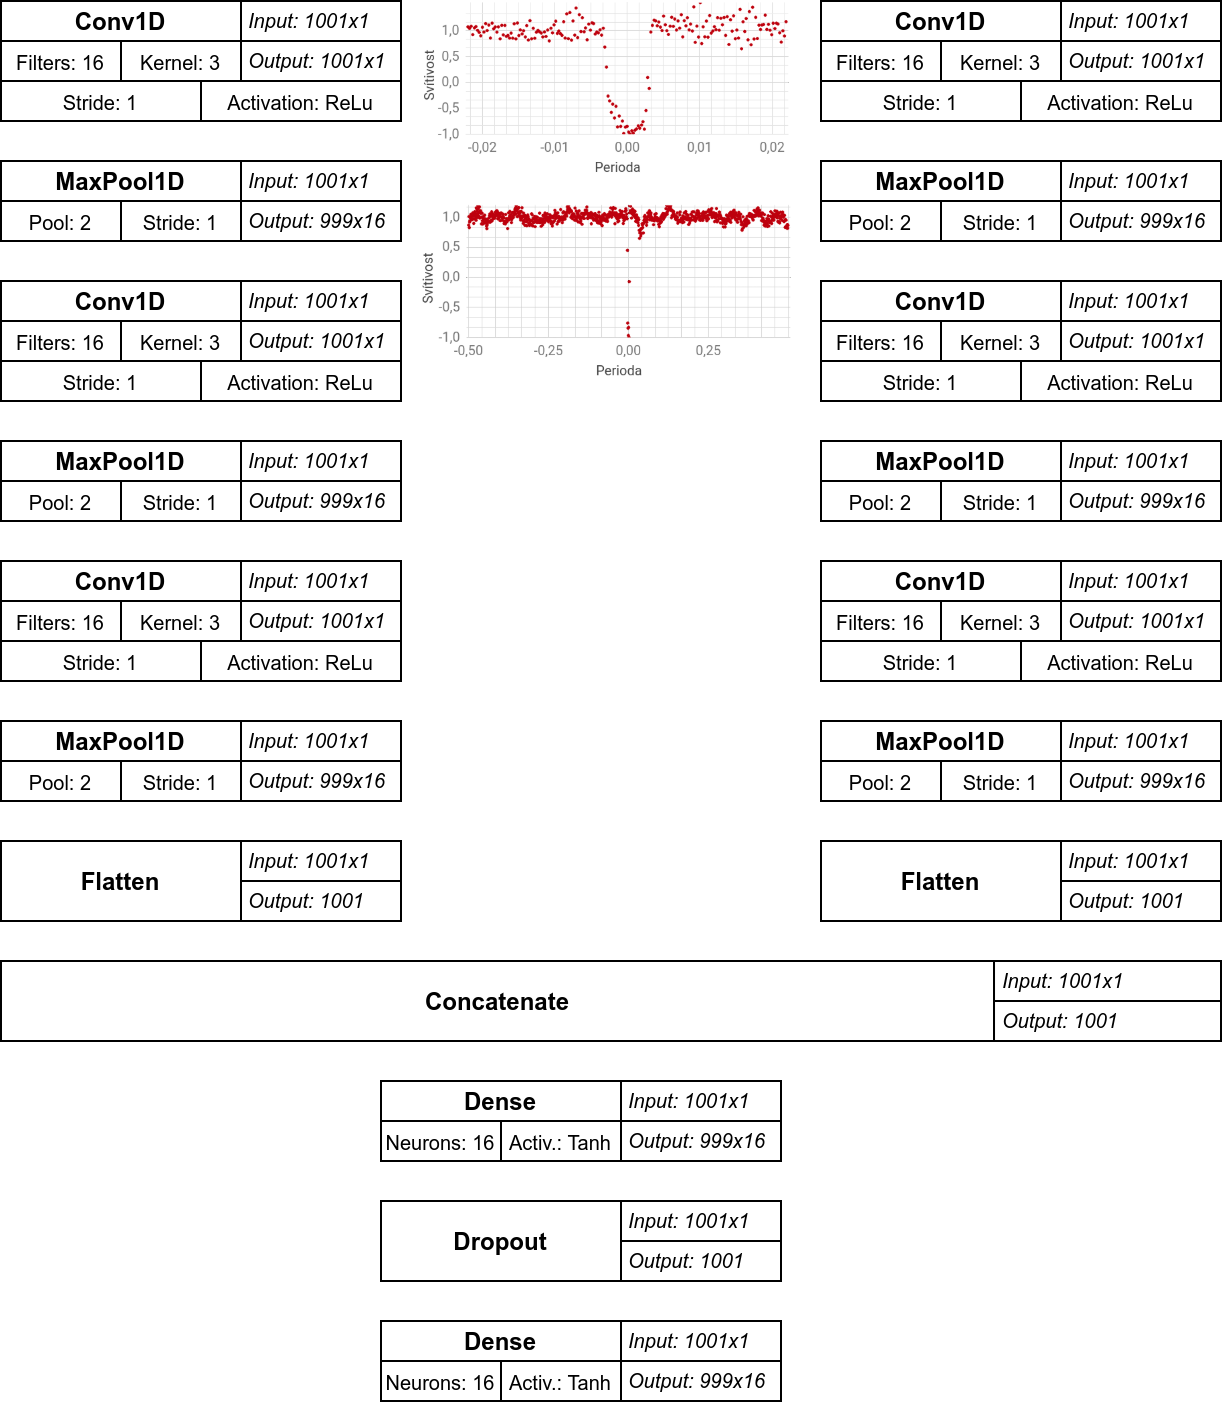
\includegraphics[width=\linewidth]{img/lc_cnn.png}

\section*{Příloha~B -- Architektura databáze}\label{priloha_b}
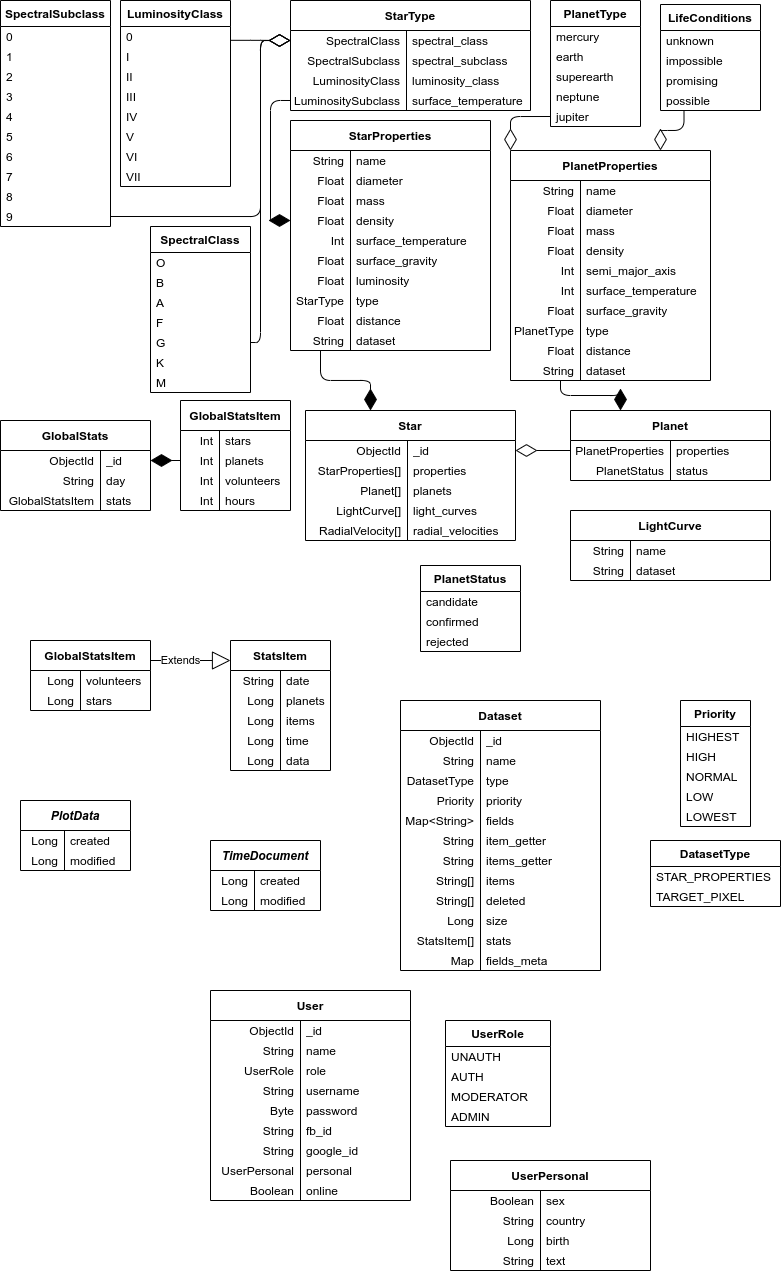
\includegraphics[width=\linewidth]{img/db.png}

\end{document}